\documentclass{llncs}
\usepackage{latexsym}
\usepackage{times}
\usepackage{amsmath}
\usepackage{graphicx}
\usepackage{tikz}
\usepackage{pgfplots}
\usepackage{cite}
\usepackage{booktabs}
\usepackage{adjustbox}
\usepackage{marvosym}
%% Colored hyperlink 
\newcommand{\cref}[2]{\href{#1}{\color{blue}#2}}
%% Colored hyperlink showing link in TT font
% \newcommand{\chref}[1]{\href{#1}{\small\tt \color{blue}#1}}
\newcommand{\hcref}[1]{\cref{#1}{\small\tt #1}}

\bibliographystyle{splncs04}
%\bibliographystyle{abbrv}

\newcommand{\one}{\mbox{\bf 1}}
\newcommand{\zero}{\mbox{\bf 0}}
\newcommand{\leafone}{L_1}
\newcommand{\leafzero}{L_0}
\newcommand{\booland}{\land}
\newcommand{\boolor}{\lor}
\newcommand{\pand}{\mathbin{\land_{\rm pv}}}
\newcommand{\por}{\mathbin{\lor_{\rm pa}}}
\newcommand{\boolxor}{\oplus}
\newcommand{\boolnot}{\neg}
%\newcommand{\tautology}{\top}
%\newcommand{\nil}{\bottom}
\newcommand{\tautology}{1}
\newcommand{\nil}{0}
\newcommand{\obar}[1]{\overline{#1}}
\newcommand{\ite}{\mbox{\it ITE}}

\newcommand{\opname}[1]{\mbox{\sc #1}}
\newcommand{\andop}{\opname{And}}
\newcommand{\implyop}{\opname{Imply}}

\newcommand{\turnstile}{\vdash}

\newcommand{\fname}[1]{\mbox{\small\sf #1}}

\newcommand{\lo}{\fname{Lo}}
\newcommand{\hi}{\fname{Hi}}
\newcommand{\var}{\fname{Var}}
\newcommand{\val}{\fname{Val}}

\newcommand{\makenode}[1]{{\mathbf #1}}
\newcommand{\nodeu}{\makenode{u}}

\newcommand{\interp}{\alpha}
\newcommand{\interpset}[1]{{\cal M}(#1)}
\newcommand{\ring}{{\cal Z}}
\newcommand{\cost}{\sigma}
\newcommand{\density}{\rho}
\newcommand{\hashset}{{\cal H}}
\newcommand{\fhash}{h}
\newcommand{\mcount}{\mu}

\newcommand{\ifarg}{\textbf{I}}
\newcommand{\thenarg}{\textbf{T}}
\newcommand{\elsearg}{\textbf{E}}
\newcommand{\depend}{{\it D}}

\newcommand{\subs}[2]{[#2/#1]}
\newcommand{\substrue}[1]{\subs{#1}{\tautology}}
\newcommand{\subsfalse}[1]{\subs{#1}{\false}}

\newcommand{\subspace}{{\cal S}}

\title{Notes on Validated Model Counting \\ Version of \today}

\author{Randal E. Bryant}

\authorrunning{R. E. Bryant}

\titlerunning{Validated Model Counting}


\institute{
Computer Science Department \\
Carnegie Mellon University, Pittsburgh, PA, United States
}

\begin{document}

\maketitle

\section{Notation}

Let $X = \{x_1, x_2, \ldots, x_n\}$ be a set of Boolean variables.  An
{\em assignment} is a function $\interp$ assigning Boolean values to
the variables: $\interp:X \rightarrow \{\nil, \tautology\}$.  We can
also view an assignment as a set of {\em literals} $\{l_1, l_2,
\ldots, l_n\}$, where each literal $l_i$ is either $x_i$ or
$\obar{x}_i$, corresponding to the assignments $\interp(x_i)$ = 1 or 0,
respectively.

\subsection{Boolean Functions}

A {\em Boolean function} $f:2^X \rightarrow \{0,1\}$ can be
characterized by the set of assignments for which the function
evaluates to 1: $\interpset{f} = \{ \interp | f(\interp) = 1\}$.  Let
$\one$ denote the Boolean function that assigns value 1 to every
assignment, and $\zero$ denote the assignment that assigns value 0 to
every assignment.  These are characterized by the universal and empty
assignment sets, respectively.


From
this we can define the {\em complement} of function $f$ as the function
$\boolnot f$ such that
$\interpset{\boolnot f} = \{ \interp | f(\interp) = 0\}$.
We can also define the conjunction and disjunction operations over functions $f_1$ and $f_2$ as characterized by the sets
$\interpset{f_1 \booland f_2} = \interpset{f_1} \cap \interpset{f_2}$ and
$\interpset{f_1 \boolor f_2} = \interpset{f_1} \cup \interpset{f_2}$.

For assignment $\interp$ and a Boolean formula $E$ over $X$, we
use the notation $\interp\subs{x_i}{E}$ to denote the assignment
$\interp'$, such that $\interp'(x_j) = \interp(x_j)$ for all $j \not = i$
and $\interp'(x_i) = \interp(E)$, where $\interp(E)$ is the value obtained by evaluating formula $E$ with each variable assigned the value given by $\interp$.
In particular, the notation
$\interp(\subs{x_i}{\obar{x}_i})$
indicates the assignment in which the value
assigned to $x_i$ is complemented, while others remain unchanged.

A Boolean function $f$ is said to be {\em independent} of variable
$x_i$ if every $\interp \in \interpset{f}$ has $\interp(\subs{x_i}{\obar{x}_i})
\in \interpset{f}$.  The {\em dependency set} of $f$, denoted
$\depend(f)$ consists of all variables $x_i$ for which $f$ is {\em
  not} independent.

\subsection{Separable Cost Functions}

Let $\ring$ denote the elements of a commutative ring.  A {\em
  separable cost function} $\cost:X \rightarrow \ring$ assigns a value
from the ring to each variable.  We extend this function by defining
the cost of literal $\obar{x}_i$ as $\cost(\obar{x}_i) = 1 - \cost(x_i)$, the cost
of an assignment as $\cost(\interp) = \prod_{l_i \in \interp}
\cost(l_i)$, and the cost of a function $f$ as $\cost(f) =
\sum_{\interp \in \interpset{f}} \cost(\interp)$.

{\bf Example 1}: Let $\ring$ be the set of rational numbers and
$\cost(x_i) = 1/2$ for all variables $x_i$.  The cost of every
assignment is then $1/2^{n}$, and the cost of a function is its
{\em density}, denoted $\density(f)$.  That is, the density of $f$ satisfies
$0 \leq \density(f) \leq 1$.  It
is the fraction of assignments for which the $f$
evaluates to 1, with $\density(\zero) = 0$ and $\density(\one) = 1$.  The density of a function
$f$ can be scaled by $2^n$ to compute the total number of models
$|\interpset{f}|$.  This is the core task of model counting.  Using
density as the metric, rather than the number of models, has the advantage that it does not vary when the
function is embedded in a larger domain $X' \supseteq X$.  As a
variant, some other forms of weighted model counting can be supported by
assigning weights of the form $\cost(x_i) = w_i$, where $0 \leq w_i
\leq 1$ for every variable $x_i$.

{\bf Example 2}: Let $\ring$ be a field with $|\ring| > 2n$,
and let $\hashset$ be the set of functions
mapping elements of $X$ to elements of $\ring$.  For
two distinct functions $f_1$ and $f_2$ and a randomly chosen $\fhash
\in \hashset$, the probability that $h(f_1) = h(f_2)$ will be at most
$2^n/|\ring|< 1/2$.  Therefore, these functions can be used as part of a
randomized algorithm for equivalence testing~\cite{blum:ipl:1980}.

\subsection{Computing Cost Functions}

Three key properties of separable cost functions make it possible, in
some cases, to compute the cost of a Boolean formula without
enumerating all of its satisfying solutions.


\begin{lemma}[Complementation]
\label{lemma:complementation}
  For separable cost function $\cost$ and Boolean function $f$:
  $\cost(\neg f) = 1 - \cost(f)$.
\end{lemma}

\begin{lemma}[Variable-Partitioned Conjunction]
\label{lemma:conjunction}
  For separable cost function $\cost$ and Boolean functions $f_1$ and $f_2$ such that $\depend(f_1) \cap \depend(f_2) = \emptyset$:
    $\cost(f_1 \land f_2) = \cost(f_1) \cdot \cost(f_2)$.
\end{lemma}
We use the notation $f_1 \pand f_2$ to denote the conjunction of $f_1$ and
$f_2$ under the condition that $f_1$ and $f_2$ are defined over
disjoint sets of variables.

\begin{lemma}[Assignment-Partitioned Disjunction]
\label{lemma:disjunction}
  For separable cost function $\cost$ and Boolean functions $f_1$ and $f_2$ such that $\interpset{f_1} \cap \interpset{f_2} = \emptyset$:
    $\cost(f_1 \lor f_2) = \cost(f_1) + \cost(f_2)$.
\end{lemma}
We use the notation $f_1 \por f_2$ to denote the disjunction of $f_1$ and $f_2$ under the
condition that $f_1$ and $f_2$ hold for mutually exclusive assignments.

\section{Proof Framework for Cost Functions}

We introduce the CRAT clausal proof framework for generating a
checkable proof of the valuation of a Boolean formula, given in
conjunctive normal form, according to a specified cost function.  A
CRAT proof provides two forms of information: 1) a {\em schema} for computing a cost
function using the ring operations, and 2) a {\em proof} that this schema
accurately characterizes the cost function for the input formula.
A schema can be either {\em function independent}, meaning that it holds
for any cost function, or {\em function dependent}, meaning that
it holds for only for a specific cost function.

The CRAT format draws its inspiration from the LRAT format for Boolean formulas and the
QRAT format for
quantified Boolean formulas (QBF).  The following are its key properties:
\begin{itemize}
\item As with LRAT, a clause can be added as long as either 1) it is
  blocked, or 2) it satisfies the RUP/RAT property with respect to a supplied sequence
  of earlier antecedent clauses.
\item  Extension variables can be introduced only according to the operations $\pand$, $\por$, and to an abstraction rule.
\begin{itemize}
\item The checker tracks the dependency set for every input and
  extension variable.  When an extension variable is introduced based
  on the $\pand$ operation, the dependency sets of its arguments must
  be disjoint.
\item When an extension variable is introduced based on the $\por$
  operation, the step must cite earlier steps providing a RUP/RAT proof
  that the two arguments are mutually exclusive.
\item The {\em abstraction} operation allows an extension
  variable to serve as an alias for one of more other 
  variables.  Use of this rule renders the schema function dependent.
\item Boolean complement is provided implicitly by allowing the
  arguments of the extension operations to be literals and not just
  variables.
\end{itemize}
\item Unlike LRAT, the deletion of a clause requires showing that this clause is implied by one or more other clauses.
\item Unlike QRAT, it need not support universal quantification.
\end{itemize}

\subsection{Syntax}

\begin{table}
  \caption{CRAT Step Types.  $C$: clause identifier, $L$: literal, $V$: variable}
  \label{tab:crat:syntax}
\centering{
  \begin{tabular}{lllll}
    \multicolumn{4}{c}{Rule} & \multicolumn{1}{c}{Description} \\
    \midrule
    \makebox[5mm][l]{$C$} & \makebox[7mm][l]{\tt i}  & \makebox[15mm][l]{$L^{*}$ {\tt 0}} & \makebox[15mm][l]{}  & \makebox[20mm][l]{Input clause} \\
    $C$ & {\tt ab} & $L^{+}$ {\tt 0} & ${\tt -}C^{*}$  {\tt 0}  & Add blocked clause \\
    $C$ & {\tt ar} & $L^{*}$ {\tt 0} & $C^{+}$  {\tt 0} & Add RUP/RAT clause \\
     & {\tt dr} & $C$             & $C^{+}$  {\tt 0} & Delete RUP/RAT clause \\
    \midrule
        & {\tt p} & $V \; L \; L$    &                  & Declare $\pand$ operation \\
        & {\tt s} & $V \; L \; L$    & $C^{+}$ {\tt 0}  & Declare $\por$ operation \\ 
        & {\tt a} & $V \; L$         & $V^{+}$ {\tt 0}  & First application of abstraction \\ 
        & {\tt a} & $V \; L$         &                  & Subsequent applications of abstraction \\ 
  \end{tabular}
  }
\end{table}

Table~\ref{tab:crat:syntax} shows the set of proof rules for the CRAT
format.  As with other clausal proof formats, a variable is
represented by a positive integer $v$, with the first ones being input
variables and successive ones being extension variables.  Literal $l$
is represented by a signed integer, with $-v$ being the complement of
variable $v$.  Each clause is indicated by a positive integer
identifier $C$, with the first ones being input clauses and successive
ones being added clauses.  Clause identifiers must be totally ordered,
such that clause $C$ can only reference clauses $C'$ such that $C' <
C$.  However, clause identifiers need not be consecutive.

The first set of proof rules are similar to those in other clausal
proofs.  Our syntax optionally allows input clauses to be listed with
a rule of type {\tt i}.  Clauses can be added via
blocked-clause and RUP/RAT rules.  The hints portion of a
blocked-clause addition lists all earlier clauses containing
the negated version of the pivot literal, with the clause IDs negated.  The hints portion of a
resolution addition must contain a sequence of clause IDs such that
the added clause is RUP/RAT with respect to these clauses.  Clause
deletion requires an explicit justification that the deleted clauses
is RUP/RAT with respect to other clauses.

The second set of proof rules is unique to the CRAT format.  Each of
these indicates the addition of an extension variable.  For each case,
the rule must be followed by a sequence of blocked-clause additions.
A product rule of the form ${\tt p}\;v\;l_1\;l_2$ indicates that $v$
will represent the product $l_1 \pand l_2$.  The blocked clause
additions must encode the formula $v \leftrightarrow (l_1 \land l_2)$.
Literals $l_1$ and $l_2$ must have disjoint dependency sets.

A sum rule of the form ${\tt s}\;v\;l_1\;l_2$ indicates that $v$ will
represent the disjunction $l_1 \por l_2$.  The blocked clause
additions must encode the formula $v \leftrightarrow (l_1 \lor l_2)$.
The rule also contains a sequence of clause IDs such that the clause
$\obar{l}_1 \lor \obar{l}_2$ is RUP/RAT with respect to the sequence.

An abstraction rule of the form ${\tt a}\;v\;l$ indicates that
variable $v$ will be an alias for literal $l$.  The syntax differs
according to whether or not this is the first use of $v$ as an
alias.  The first instance must include a list of variables that is a
(possibly improper) superset of the dependency set for $l$.  It must
be followed by a sequence of blocked-clause additions encoding the
formula $v \leftrightarrow l$.  Subsequent instances do not
include an explicit dependency set, but $\depend(l)$ must be a subset of
those declared for $v$.  Furthermore, there are no blocked-clause
additions for these cases.


\subsection{Semantics}

A CRAT proof follows the same general form as a QRAT dual proof---one
that ensures that each clause addition and each clause deletion preserves
equivalence.  Starting with the set of input clauses, it produces a
sequence of steps that both add and delete clauses.  Each addition
must be truth preserving and each deletion must be falsehood
preserving.  At the end, all input clauses must have been deleted, and
among the remaining clauses there must be only a single unit clause consisting of some variable or
its complement.  Except for trivial cases, the final variable will be
an extension variable.  The sequence of extension operations define
the schema for computing the cost function.  That is, a value for the
cost function is computed for every literal according to the rules of
Lemmas \ref{lemma:complementation}--\ref{lemma:disjunction}.  For
every abstraction step, all literals having the indicated extension
variable as their alias must evaluate to the same value.  The computed
cost is then the value computed for the literal in the final unit
clause.

\subsection{Example}

\begin{figure}
  \centering{
    \begin{minipage}{0.4\textwidth}
      A) Logical Form   \\[2ex]
    \centering{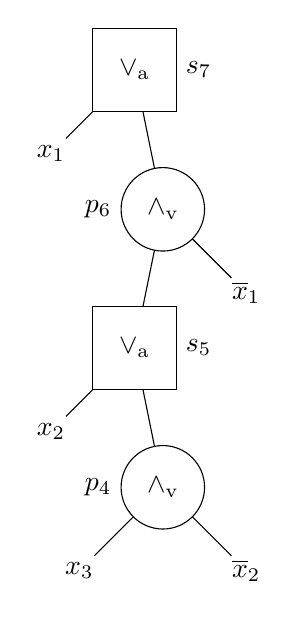
\begin{tikzpicture}
\definecolor{neutralcolor}{RGB}{0,0,0}
\definecolor{pathcolor}{RGB}{0,0,0}
\definecolor{fillcolor}{RGB}{255,255,255}
\definecolor{background}{RGB}{225,225,225}
\definecolor{highcolor}{RGB}{0,0,0}
\definecolor{lowcolor}{RGB}{0,0,0}
\draw (1.32,6.62) [thin,neutralcolor] -- (0.26,5.56);
\draw (1.32,6.62) [thin,neutralcolor] -- (1.68,4.85);
\draw (1.68,4.85) [thin,neutralcolor] -- (2.74,3.79);
\draw (1.68,4.85) [thin,neutralcolor] -- (1.32,3.09);
\draw (1.32,3.09) [thin,neutralcolor] -- (0.26,2.03);
\draw (1.32,3.09) [thin,neutralcolor] -- (1.68,1.32);
\draw (1.68,1.32) [thin,neutralcolor] -- (2.74,0.26);
\draw (1.68,1.32) [thin,neutralcolor] -- (0.62,0.26);
\draw [thin,fill=fillcolor,draw=neutralcolor] (1.68,4.85) circle [radius=0.53];
\node at (1.68,4.85) {$\mathbin{\land_{\textrm{v}}}$};
\draw [thin,fill=fillcolor,draw=neutralcolor] (1.68,1.32) circle [radius=0.53];
\node at (1.68,1.32) {$\mathbin{\land_{\textrm{v}}}$};
\draw [thin,fill=fillcolor,draw=fillcolor] (2.74,0.26) circle [radius=0.26];
\node at (2.74,0.26) {$\overline{x}_2$};
\draw [thin,fill=fillcolor,draw=neutralcolor] (0.79,6.09) rectangle (1.85,7.15);
\node at (1.32,6.62) {$\mathbin{\lor_{\textrm{a}}}$};
\draw [thin,fill=fillcolor,draw=neutralcolor] (0.79,2.56) rectangle (1.85,3.62);
\node at (1.32,3.09) {$\mathbin{\lor_{\textrm{a}}}$};
\draw [thin,fill=fillcolor,draw=fillcolor] (2.74,3.79) circle [radius=0.26];
\node at (2.74,3.79) {$\overline{x}_1$};
\draw [thin,fill=fillcolor,draw=fillcolor] (0.26,2.03) circle [radius=0.26];
\node at (0.26,2.03) {$x_2$};
\draw [thin,fill=fillcolor,draw=fillcolor] (0.62,0.26) circle [radius=0.26];
\node at (0.62,0.26) {$x_3$};
\draw [thin,fill=fillcolor,draw=fillcolor] (0.26,5.56) circle [radius=0.26];
\node at (0.26,5.56) {$x_1$};
\node [right] at (1.85,6.62) {$s_7$};
\node [left] at (1.15,4.85) {$p_6$};
\node [right] at (1.85,3.09) {$s_5$};
\node [left] at (1.15,1.32) {$p_4$};
\end{tikzpicture}%%
}
    \end{minipage}
    \begin{minipage}{0.4\textwidth}
    B) Evaluation Form\\[2ex]
    \centering{\begin{tikzpicture}
\definecolor{neutralcolor}{RGB}{0,0,0}
\definecolor{pathcolor}{RGB}{0,0,0}
\definecolor{fillcolor}{RGB}{255,255,255}
\definecolor{background}{RGB}{225,225,225}
\definecolor{highcolor}{RGB}{0,0,0}
\definecolor{lowcolor}{RGB}{0,0,0}
\draw (1.32,6.80) [thin,neutralcolor] -- (0.26,5.74);
\draw (1.32,6.80) [thin,neutralcolor] -- (1.68,5.03);
\draw (1.68,5.03) [thin,neutralcolor] -- (2.74,3.97);
\draw (1.68,5.03) [thin,neutralcolor] -- (1.32,3.27);
\draw (1.32,3.27) [thin,neutralcolor] -- (0.26,2.21);
\draw (1.32,3.27) [thin,neutralcolor] -- (1.68,1.50);
\draw (1.68,1.50) [thin,neutralcolor] -- (2.74,0.44);
\draw (1.68,1.50) [thin,neutralcolor] -- (0.62,0.44);
\draw [thin,fill=fillcolor,draw=fillcolor] (1.68,5.03) circle [radius=0.26];
\node at (1.68,5.03) {{\texttt{*}}};
\draw [thin,fill=fillcolor,draw=fillcolor] (1.68,1.50) circle [radius=0.26];
\node at (1.68,1.50) {{\texttt{*}}};
\draw [thin,fill=fillcolor,draw=fillcolor] (2.74,0.44) circle [radius=0.44];
\node at (2.74,0.44) {$1-w_2$};
\draw [thin,fill=fillcolor,draw=fillcolor] (1.32,6.80) circle [radius=0.26];
\node at (1.32,6.80) {{\texttt{+}}};
\draw [thin,fill=fillcolor,draw=fillcolor] (1.32,3.27) circle [radius=0.26];
\node at (1.32,3.27) {{\texttt{+}}};
\draw [thin,fill=fillcolor,draw=fillcolor] (2.74,3.97) circle [radius=0.44];
\node at (2.74,3.97) {$1-w_1$};
\draw [thin,fill=fillcolor,draw=fillcolor] (0.26,2.21) circle [radius=0.26];
\node at (0.26,2.21) {$w_2$};
\draw [thin,fill=fillcolor,draw=fillcolor] (0.62,0.44) circle [radius=0.26];
\node at (0.62,0.44) {$w_3$};
\draw [thin,fill=fillcolor,draw=fillcolor] (0.26,5.74) circle [radius=0.26];
\node at (0.26,5.74) {$w_1$};
\node [right] at (1.59,6.80) {$s_7$};
\node [left] at (1.41,5.03) {$p_6$};
\node [right] at (1.59,3.27) {$s_5$};
\node [left] at (1.41,1.50) {$p_4$};
\end{tikzpicture}%%
}
    \end{minipage}
  }
\caption{Schema for Formula $x_1 \lor x_2 \lor x_3$}
\label{fig:c3:schema}
\end{figure}

\begin{figure}
  \centering{
  \begin{tabular}{llllll}
    \multicolumn{4}{c}{Proof line} & & \multicolumn{1}{c}{Explanation} \\
\midrule
    \makebox[5mm][l]{\tt 1} & \makebox[7mm][l]{\tt i}   & \makebox[20mm][l]{\tt 1 2 3 0}   &  \makebox[15mm]{}          & \makebox[5mm]{} & \makebox[20mm][l]{Input clause}\\
            & {\tt p}   & {\tt 4 -2 3}  &            & & Declare $p_4 = \obar{x}_2 \pand x_3$ \\
    {\tt 2} & {\tt ab}  & {\tt 4  2 -3 0}  & {\tt 0}    & & Defining clauses for $p_4$ \\ 
    {\tt 3} & {\tt ab}  & {\tt -4 -2 0}    & {\tt -2 0} & & \\ %%Defining clause for $p_4$ \\ 
    {\tt 4} & {\tt ab}  & {\tt -4 3 0}    & {\tt -2 0} & & \\ %%Defining clause for $p_4$ \\ 
            & {\tt s}   & {\tt 5 2 4}   & {\tt 3 0}  & & Declare $s_5 = x_2 \por p_4$ \\
    {\tt 5} & {\tt ab}  & {\tt -5 2 4 0}  & {\tt 0}    & & Defining clauses for $s_5$ \\ 
    {\tt 6} & {\tt ab}  & {\tt  5 -2 0}    & {\tt -5 0} &  \\  %%Defining clause for $s_5$ \\ 
    {\tt 7} & {\tt ab}  & {\tt  5 -4 0}    & {\tt -5 0} & &  \\  %%Defining clause for $s_5$ \\ 
            & {\tt p}   & {\tt 6 -1 5}  &            & & Declare $p_6 = \obar{x}_1 \pand s_5$ \\
    {\tt 8} & {\tt ab}  & {\tt 6  1 -5 0}  & {\tt 0}    & & Defining clauses for $p_6$ \\ 
    {\tt 9} & {\tt ab}  & {\tt -6 -1 0}    & {\tt -8 0} & &  \\  %%Defining clause for $p_6$ \\ 
    {\tt 10} & {\tt ab}  & {\tt -6 5 0}    & {\tt -8 0} & &  \\  %%Defining clause for $p_6$ \\ 
             & {\tt s}   & {\tt 7 1 6}   & {\tt 9 0}  & & Declare $s_7 = x_1 \por p_6$ \\
    {\tt 11} & {\tt ab}  & {\tt -7 1 6 0}  & {\tt 0}    & & Defining clauses for $s_7$ \\ 
    {\tt 12} & {\tt ab}  & {\tt  7 -1 0}    & {\tt -12 0} & &  \\  %%Defining clause for $s_7$ \\ 
    {\tt 13} & {\tt ab}  & {\tt  7 -6 0}    & {\tt -12 0} & &  \\  %%Defining clause for $s_7$ \\ 
    {\tt 14} & {\tt ar}  & {\tt 7 0} & {\tt 12 13 7 6 2 1 0} & & Assert unit clause $[s_7]$ \\
             & {\tt dr}  & {\tt 1}  & {\tt 4 5 10 11 14 0} & & Delete input clause \\
  \end{tabular}
  }
  \caption{CRAT Proof Steps for Formula $x_1 \lor x_2 \lor x_3$}
  \label{fig:c3:crat}
\end{figure}
    
As an illustration, consider the Boolean formula $x_1 \lor x_2 \lor
x_3$, represented by a single clause.  We cannot directly use the
$\por$ operation to form these disjunctions, since the sets of assignments
satisfying the individual literals are not disjoint.  Instead, we must
decompose this formula into a sequence of operations, as shown by the
logical form of Figure~\ref{fig:c3:schema}A\@.  Circles in this schema
correspond to $\pand$ operations and squares to $\por$ operations.
The subscripts of the variables and the operator labels correspond to
the numbers of the input and extension variables in the CRAT proof.

The conjunction of $\obar{x}_2$ and $x_3$ can be computed as $p_4 =
\obar{x}_2 \pand x_3$, since the literals have disjoint dependency
sets. We can then express the disjunction $x_2 \lor x_3$ as
as $s_5 = x_2 \por p_4$.  A similar process forms the
disjunction $x_1 \lor x_2 \lor x_3$ by first forming the product $p_6
= \obar{x}_1 \pand s_5$ and the final sum $s_7 = x_1 \por p_6$.

The logical representation can readily be converted into a schema for
computing the cost of the formula, given weight $w_i$ for each
variable $x_i$ for $1 \leq i \leq 3$.  This is illustrated in
Figure~\ref{fig:c3:schema}B\@.  This schema is valid for any cost
function, since it contains no abstraction operations.

Figure~\ref{fig:c3:crat} shows an annotated version of the CRAT proof
for this example.  Clause \#1 corresponds to the input formula, and
clauses \#2--\#13 are the defining clauses for the four operations.
Each of the two sum operations lists one of the earlier defining
clauses as a proof that its arguments are mutually exclusive.
Clause \#14 adds the unit clause corresponding to sum $s_7$,
indicating that the extension variable variable will evaluate to
$\tautology$  for any assigment that satisfies the input clause.  We
can write this as $C \turnstile s_7$ for input clause $C$.  The
deletion step at the end turns this around, showing that $s_7
\turnstile C_I$, and therefore the input clause can be deleted, This
completes a proof that extension variable $s_7$ is logically
equivalent to the input formula.

\section{Looking Ahead}

\subsection{Implementing Certified Counters}

Given an arbitrary CNF formula, we can use BDD operations to generate
a schematic representation.  The proof generation can follow the
methods we have used for generating unsatisfiability proofs of Boolean
formulas~\cite{bryant:tacas:2021} and dual proofs of quantified
Boolean formulas~\cite{bryant:cade:2021}.  The key idea 
is to use extended resolution to encode the semantics of the BDD
nodes as part of the proof.  Here we can further decompose each $\ite$
(short for ``if-then-else'') operation representing a BDD node into
two $\pand$ and one $\por$ operation.  That is, we can encode
$\ite(x,A,B)$ as $(x \pand A) \por (\obar{x} \pand B)$, where $x$ is an
input variable and $A$ and $B$ are subformulas.  The sum operation trivially satisfies the disjoint assignment requirement, since $x$ has positive polarity in the first product and negative polarity in the second.
We must also
make sure that $x$ is not in the dependency set of either $A$ or $B$.
For ordered BDDs,~\cite{Bryant:1986} this property holds, because the
variables in $A$ and $B$ will be greater in the variable ordering than
$x$.

The BDD representations of many of the formulas occuring in
model-counting problems are far to large for this approach to be
practical.  One refinement of the approach, implemented by the ADDMC
model counter, is to abstract subformulas, keeping track only of the
number of models they can have and representing a number of subformulas
with a single ADD leaf node.  Our abstraction operation is intended to
support this capability.  We can
introduce a new variable to represent the cost function for some
subformula.  If subsequent formulas are guaranteed to yield the same
cost, then these can alias to the earlier variable.  However, it is
not clear how to prove that this aliasing preserves equivalence.

Other model counters use either top-down and bottom-up methods to
generate representations of the formula that are similar to our
schmas.  These exploit the key abstractions we have identified.  We
must find ways to modify these model counters to also generate CRAT
proofs.

\subsection{TO-DO List}

\begin{itemize}
\item Proof Framework
  \begin{itemize}
  \item Generalities and details of the format
  \item What should be the final state?
  \item When can blocked clauses be deleted?
  \item How can abstraction be incorporated?
  \end{itemize}

\item Checker
  \begin{itemize}
  \item Working prototype
  \item C/C++ (or Rust?)
  \item Formally verified
  \end{itemize}

\item Counters
\begin{itemize}
\item BDD-based
  \begin{itemize}
  \item Prototype
  \item C/C++
  \end{itemize}

\item CDCL-based
  \begin{itemize}
  \item Prototype
  \item C/C++
  \end{itemize}
\end{itemize}

\end{itemize}


\bibliography{references}


\end{document}


